\chapter{Attacks on privacy} \label{section: MIA}
This chapter is devoted to investigating and evaluating attacks on machine learning models.
Differential privacy protects the centrally stored dataset from leaking sensitive information.
Therefore, assessing the mechanism's privacy is best measurable using common attacks \citep{jayaraman_evaluating_nodate}.
In this context, we evaluate attacks that explicitly uncover training data from a privately trained model.
We consider two types of attacks:
\begin{enumerate}
  \item \textbf{Membership inference attack}: An adversary attempts to infer whether a data point was used for training.
  \item \textbf{Reconstruction attack}: An adversary attempts to reconstruct the training data using the model.
\end{enumerate}
The knowledge of the attacker (adversarial knowledge) is an important factor to consider.
This knowledge can be divided into white-box and black-box approaches \citep{hu_membership_2022}.
\begin{enumerate}
  \item \textbf{White-box}: The attacker has all the needed data. Including target model parameters or the architecture \citep{hu_membership_2022}.
  \item \textbf{Black-box}: The attacker has limited information, like training data distribution and the trained model \citep{hu_membership_2022}.
\end{enumerate}
We will discuss both types of attacks and types in the next two sections.

\section{Membership inference attacks}
\todo[inline]{Formalize this}
An attack model that plays a significant role in machine learning is \gls{mia}.
With this attack, an adversary attempts to infer the training data $x \in X$ (member) from a given data point $z \in Z$ (non-member).
The attack happens exclusively on supervised learning models, which predict labels or probabilities.
Most attacks on models trained on a centralized dataset occur during the inference phase, where the trained model is used to make predictions. \citep{rigaki_survey_2021}.
This is also why we are primarily interested in this phase, as we are not using a distributed learning model.

The most well-known member inference attack is training shadow models \citep{rigaki_survey_2021}.
In this attack, an attacker trains multiple models.
These models do not necessarily have to be the same as the original model, and the focus is mainly on the data input/output.
It is a black-box attack, but the attacker often needs knowledge of the data distribution to create a good shadow dataset \citep{rigaki_survey_2021}.

One of the earlier works that used this attack was Shokri et al. \citep{shokri_membership_2017}.
An attacker trains multiple models (shadow model) to overfit the original modal.
This idea is based on the model giving higher scores to the data on which it was trained (overfitting).
Using this approach, attackers can retrieve the model's training data (member data) by injecting many fake data (non-membership data).
\begin{figure}[H]
  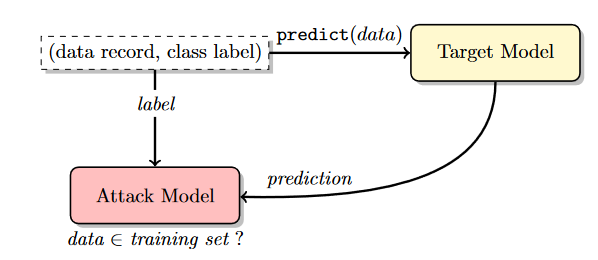
\includegraphics[width=0.5\textwidth]{TheorethicalFramework/AttacksOnPrivacy/shadow-models-mi.png}
  \caption{Black-box MIA attack on a machine learning model \citep{shokri_membership_2017}}
\end{figure}
Another approach to a black-box attack was introduced by Peng et al. and only considers that the attacker has access to the already trained model.
They first rescale the probabilities using temperature scaling to compensate for overconfident models \citep{peng_unsupervised_nodate}.
So instead of having a probability between two classes with, for example, 99\% against 1\%, it will be more evenly distributed based on the training data.
They then cluster the probabilities into two clusters using K-Means and label the higher confidence scores as members.
%Access to only the output of the model is a typical characteristic of black-box attacks. If the attacker also knows architecture, for example, it is referred to as a white-box attack.
Another take on this is prediction and confidence-based \gls{mia}, both proposed by \citep{yeom_privacy_2018}.
They assume that an attacker knows the standard error and has access to the perturbation dataset.
The algorithm can then extract the truth label by minimizing the loss. \newline
%The above attacks do rely on the model to also provide the confidence or probabilities of the predictions.
%This information is often unavailable, so Choquette-Choo et al. introduced a label-only attack.
%While the existing models exploit MIA's probability output, they rely solely on labels \citep{choquette-choo_label-only_2021}.
%They use the "HopSkipJump" attack, a so-called decision-based attack \citep{chen_hopskipjumpattack_2020}.
%Choquette-Choo et al. consider a more semi-black-box approach, for which the attacker still requires access to a subset of the original training data and the trained model.
%Another paper using "HopSkipJump" requires only the trained model and achieves higher accuracy using an approach with random data \citep{li_membership_2021}. \newline






%If the data is fed with real data the score is higher than similar data, which means the real data can be inferred \citep{shokri_membership_2017,jayaraman_evaluating_nodate}
%A white-box setting requires a lot of adversarial knowledge for training the shadow models.
%The black-box settings only take the prediction as input and decide if it is a (non-) member \citep{hu_membership_2022}.
%To conclude on this, there are many methods for MIA and in that regard, the black-box approaches look the most promising.
%They require less setup and there is plenty of black-box approaches score with a success rate of 70\% and 80\%.
%For our use case, however, it is harder to establish an MIA; as we focus mainly on clustering.
%Anyhow, it is possible if we consider a semi-supervised approach where we consider the cluster labels as ground truth.
%%Differential privacy is proposed as a wmay of solving the inference attack for both white-box and black-box \citep{hu_membership_2022}.
%%However, it is hard to find a way to protect privacy and utility as well, so it depends heavily on the privacy budget.

\newpage
\section{Reconstruction attack}
\todo[inline]{Also formalize}
The concept of reconstruction attacks predates differential privacy, as this principle also gave rise to the idea of necessary database privatization \citep{dinur_revealing_2003}.
An adversary could reconstruct training data from a given (classifier) model using a reconstruction attack.
Their research evaluates the perturbation that needs to be added to a database to protect it versus a reconstruction attack.

A general reconstruction attack for our use-case is the attribute inference attack \citep{dwork_exposed_2017} or model inference \citep{rigaki_survey_2021}.
Both terms are essentially the same, and we have chosen to name attribute inference attack, as it is the most common one in most literature \citep{jegorova_survey_2022}.
Attribute inference focuses on a reconstruction attack with the adversary's goal of retrieving the secret from each user \citep{dwork_exposed_2017}.
For example, an attacker may attempt to reconstruct information about someone's heart disease using the individual's properties.

A practical implementation of the attack was provided by Fredrikson et al. as a way to infer sensitive features \citep{fredrikson_model_2015}.
To accomplish this, they used a decision tree attack, a white-box approach, as they also accessed the count of instances for each decision tree branch.
They also considered a black-box approach with access only to the target model (ML-as-a-service in this example).
% Finally, they showed that if the attacker can capture a single output label, they can reproduce the original data with high confidence \citep{fredrikson_model_2015}.
The attack targets gradient descent, which is used to optimize the input data of an attack to mimic the original data.
It has only been shown to work on a neural network for face identification images (named MIFace) \citep{fredrikson_model_2015}, but it could be extended to another machine learning classifier if it uses gradient descent (e.g. Support Vector Machines) \citep{nicolae_adversarial_2019}.
%Most other comparable work focus almost exclusively on neural networks [decristofaroOverviewPrivacyMachine2020a, jegorovaSurveyLeakagePrivacy2022].
A more general approach was undertaken by Yeom et al., building upon the same research discussed in the previous section (Member inference).
In their work, Yeom et al. proposed a membership inference attack, which can also be utilized for attribute inference in a white-box setting.
The attribute inference attack follows a similar methodology, wherein the target model is queried to assess the loss of synthetic data based on adversarial knowledge.
Repeating the process, the attack identifies and selects the value with the highest prior probability, incorporating membership information \citep{yeom_privacy_2018,jayaraman_are_2022}.
Evaluating the effectiveness of such attacks is challenging, as it relies on the correlation between attributes, irrespective of whether the data belongs to the training or test dataset \citep{zhao_feasibility_2021}.
Therefore, Yeom et al. focus on the similarity between membership/attribute- inference and combine them to evaluate the attribute inference attack \citep{yeom_privacy_2018}. \newline

Differential privacy aims to introduce sufficient noise to mitigate the risk of various attacks \citep{dwork_exposed_2017,jayaraman_evaluating_nodate}.
Assessing the privacy leakage of our model can be effectively accomplished by employing attribute/membership inference techniques.
Within this thesis, our focus is mainly on \gls{mia}.
We aim to establish a quantifiable measure for our mechanism, and combining both attribute and membership attacks is not beneficial since they essentially capture the same information.
Therefore, it is sufficient to concentrate on membership inference attacks. %using available code implementations \citep{nicolae_adversarial_2019}.
\newpage
%\section{Model inversion attack}
%\todo[inline]{Do research for this attack}

% \section{Poison attack}
%\textbf{Reconstruction attacks:}
%Another attack that is a threat, especially to differential privacy is a reconstruction attack.
%This attack is also more known as the attribute inference attack and is more focused on the data itself than machine learning models \citep{rigaki_survey_2021}. 

%\textbf{Model extraction attacks:}
%The final attack that is considered, is the model extraction attack.
%This attack consists of the attacker being able to reconstruct and gather information about the original model.

% Jayaraman et al. evaluate inference attacks and differential privacy and express a metric called "privacy leakage"  \citep{jayaraman_evaluating_nodate}.



\section{Attack evaluation} \label{theory:attack-evaluation}
In this section, we evaluate the membership inference attack and evaluate it as it is the most appropriate for this study (See previous chapter).
We assess whether differential privacy provides protection against the attack and discuss how this can be measured.
\subsection{Member inference attacks}
% Research
Most current research for \gls{mia} is evaluated for neural networks \citep{rigaki_survey_2021}.
A tiny percentage evaluates this attack for supervised learning, with the majority using classification with decision trees.
Most studies have used a black-box approach \citep{rigaki_survey_2021} for these attacks.
This approach is not surprising, as these attacks have a high success rate and pose a greater risk of exploitation.

% Metrics
Introducing differential privacy reduces the impact of a member inference attack \citep{rigaki_survey_2021,hu_membership_2022}.
This is because the input to the model is perturbed.
While it is still possible to retrieve the training data, the leaked privacy is significantly reduced.
A simple but effective way to measure the privacy leakage is by calculating the accuracy of correctly predicting membership by the adversary \citep{choquette-choo_label-only_2021}.

Yeom et al. created a metric specifically for membership inference attacks which can be measured using an "adversarial advantage."
This metric describes the percentage of privacy compromised during a member inference attack \citep{yeom_privacy_2018}.
This metric is calculated by subtracting the \gls{fpr} from the \gls{tpr}.
The \gls{tpr} represents the number of correctly predicted member data (training data), and the \gls{fpr} represents the number of correctly predicted non-member data.
Although these metrics are commonly applied in the literature for \gls{mia}, they do not provide enough information \citep{carlini_membership_2022}.
Both metrics do not consider the imbalance between the \gls{tpr} and \gls{fpr}.
The metric should emphasize the \gls{tpr}, as this is the percentage of correctly predicted member data.
Therefore, they propose to use a ROC curve to show the effectiveness of a membership inference attack \citep{carlini_membership_2022}. \newline

% Final remark
In conclusion, the attacks that use \gls{mia} are all (mis)using supervised machine learning.
However, in this study, we use clustering algorithms.
Therefore, a semi-supervised approach can be used, as illustrated in Figure \ref{figure:MIA-semi-supervised}.
\newpage
\begin{figure}[h]
  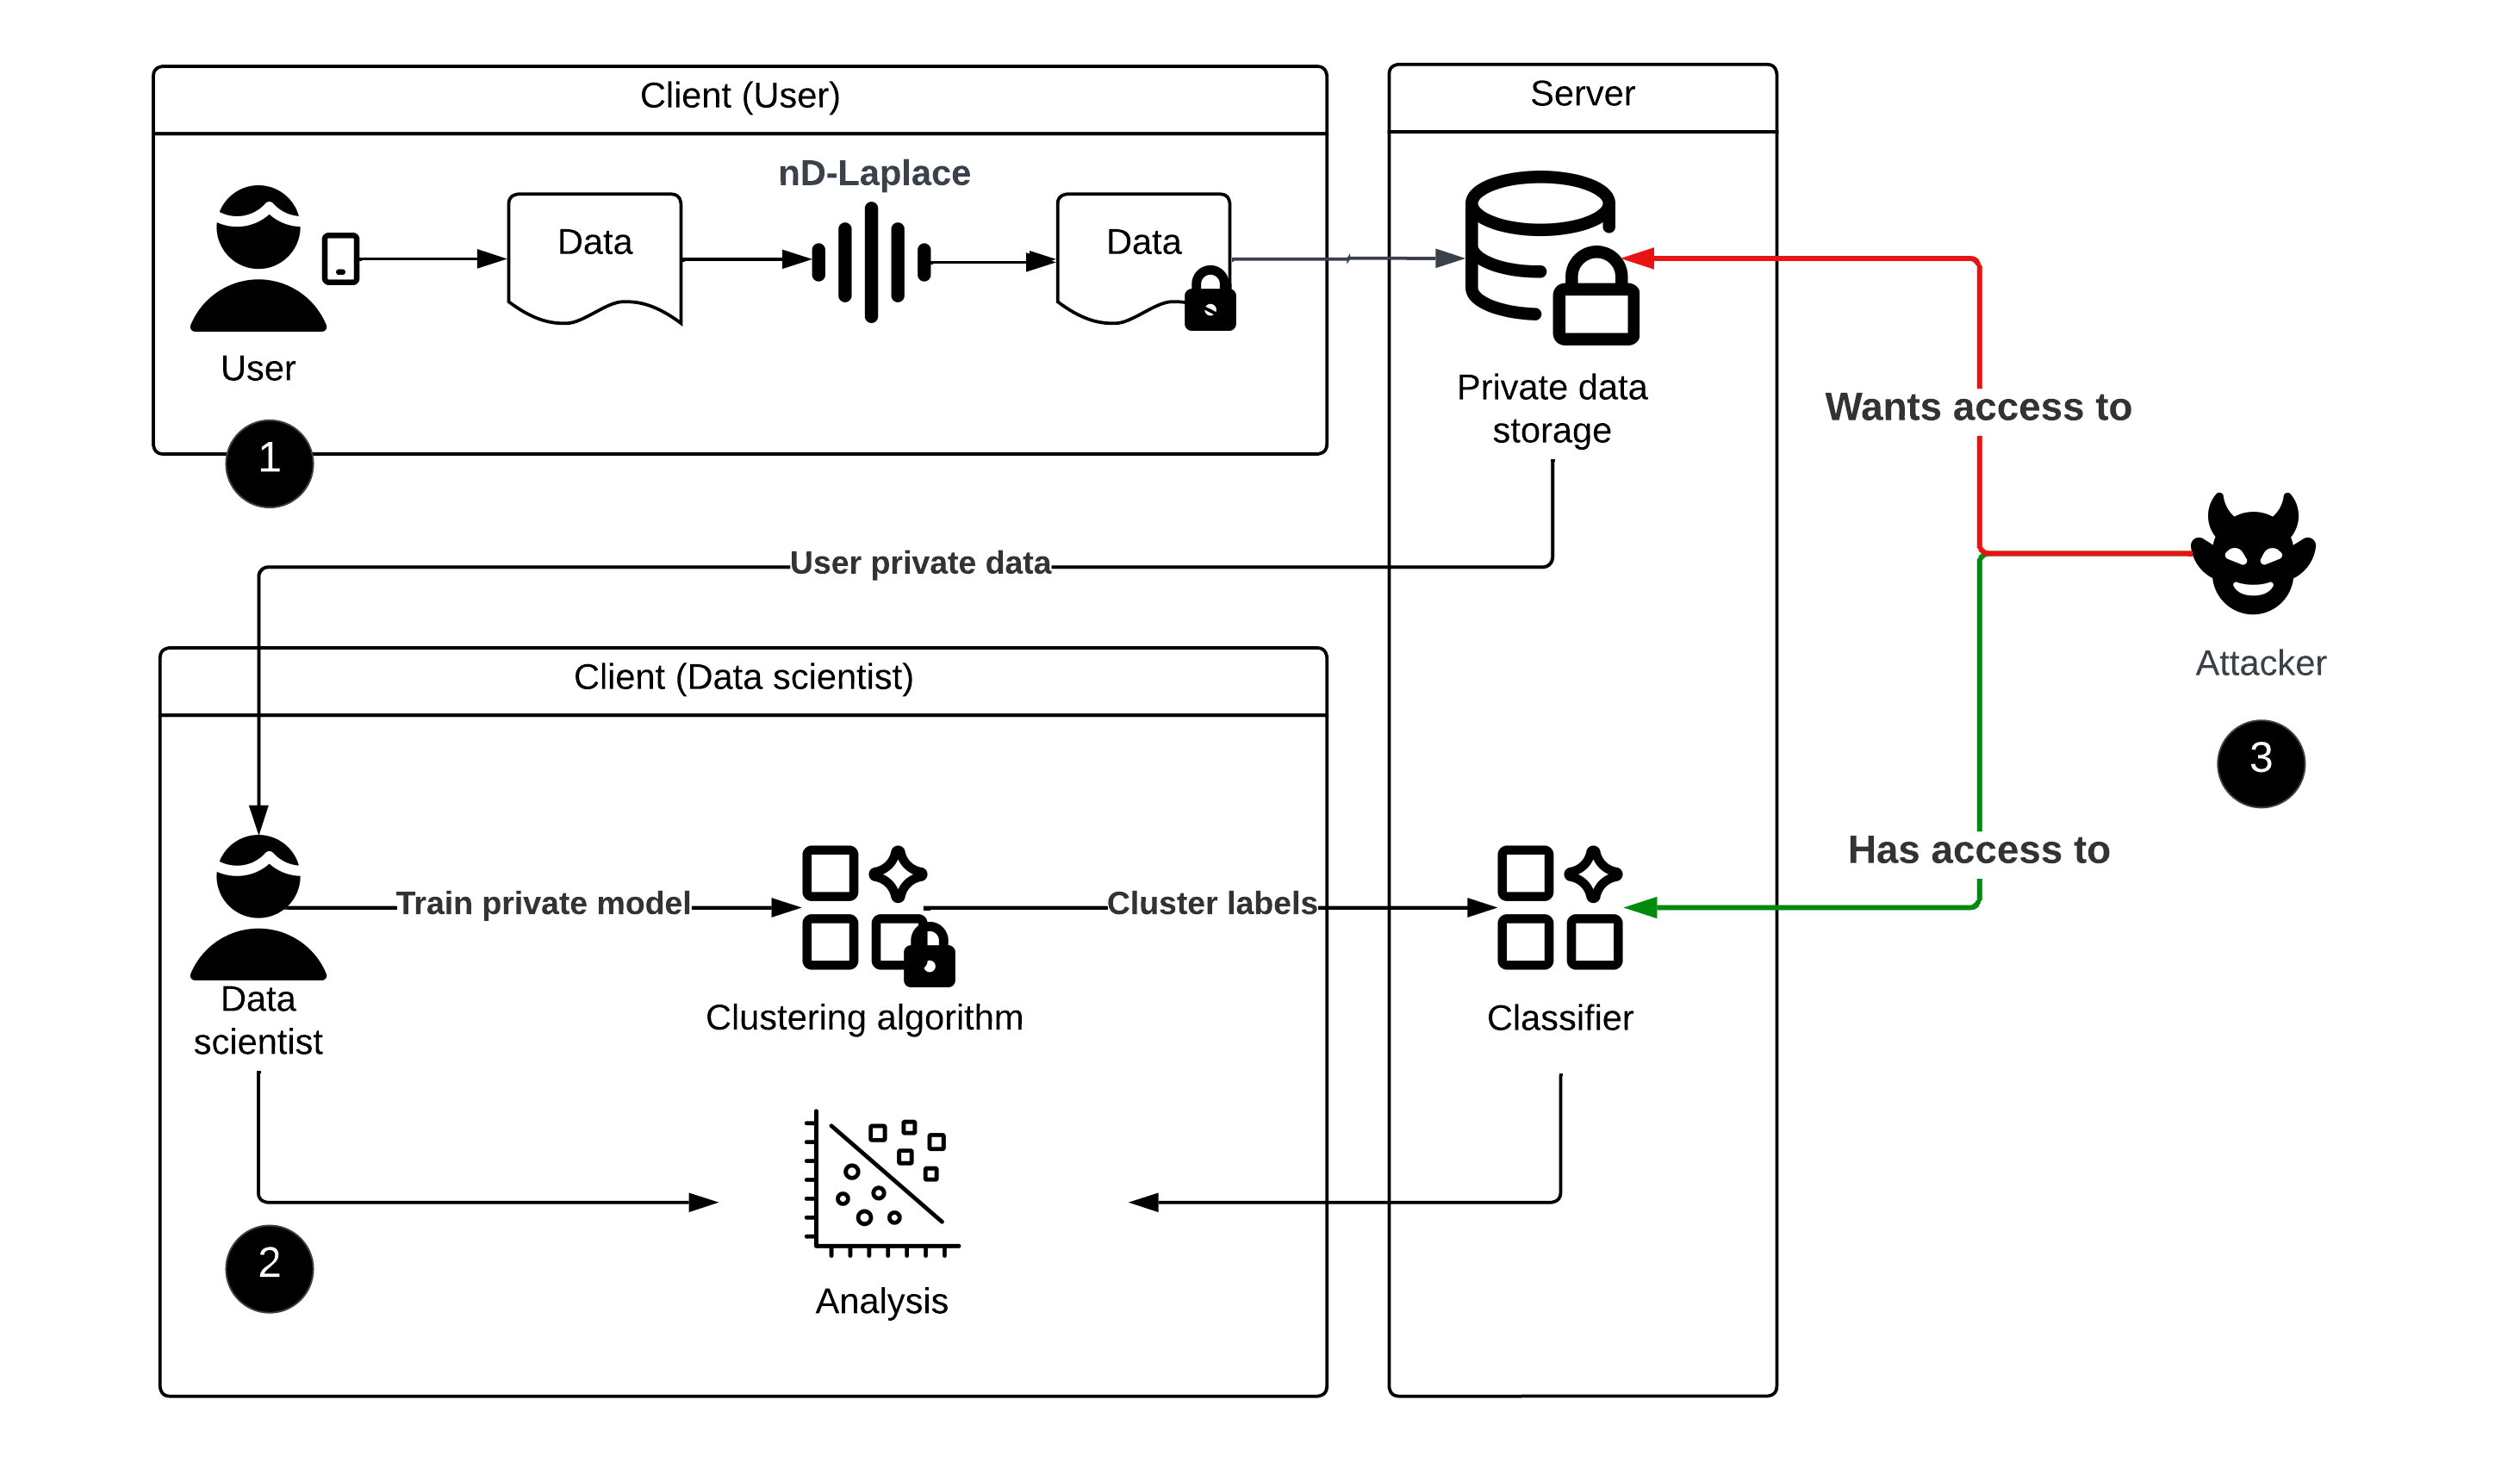
\includegraphics[width=1\textwidth]{TheorethicalFramework/Differential privacy/master-thesis-MIA.png}
  \caption{Semi-supervised black-box approach to execute a member inference attack.}
  \label{figure:MIA-semi-supervised}
\end{figure}

\begin{enumerate}
  \item The user uses a client (e.g., mobile app), where the nD-Laplace noise is added locally to the data.
  \item A data scientist trains the clustering algorithm with the privatized data.
        Therefore, the clustering algorithm's input and output (labels) are private.
        These labels are used to train a classifier (semi-supervised setup).
  \item The attacker wants access to the private data on the server.
        In this approach, the attacker has access to the classifier on the server (black-box setting).
        So, the attacker can use the classifier's output to conduct a \gls{mia}.
\end{enumerate}
